\documentclass[a4paper, 12pt]{report}
\usepackage{graphicx}
\usepackage{fancyhdr}
\usepackage{wrapfig}
\pagestyle{fancy}
\begin{document}

\graphicspath{{./images/}}
\title{Smarter and simple Scrabble strategy}
\date{Course: DD143X \\ Supervisor: Johan Boye \\ Kungliga Tekniska Högskolan \\ CSC \\ March 7, 2012}
\author{Frej Connolly \\ Götgatan 78 13TR LÄG1302 \\ 118 30 Stockholm \\ SWEDEN \\ +46(0)73-963 41 90 \\ connolly@kth.se \\
        \and Diana Gren \\ Sköldgatan 8 2TR \\ 118 63 Stockholm \\ SWEDEN \\ +46(0)70-467 47 20 \\ dianagr@kth.se}

\maketitle
\begin{abstract}
The abstract goes here.
\end{abstract}
\tableofcontents





\chapter{Introduction}
Scrabble is an old classic game, fairly easy to learn, but really difficult to be great in. How to play the game of Scrabble is a well studied problem. In comparison to other classical games such as \emph{Chess} or \emph{Checkers}, it is much more difficult to be a successful player of Scrabble due to a number of factors where the random component is considered to be the most affecting. The classic games can usually be placed in two categories; either \emph{deterministic} games och \emph{non-deterministic} games.

\begin{description}
\item[Deterministic] A game is deterministic if the players have all possible information about the state of the game, and possible future states.
\item[Non-deterministic] In contrast to a deterministic game, a non-deterministic game does not let the players now all information about the game's current or future states.
\end{description}

The main factor contributing to the difficulty of Scrabble is the randomness. Players do not have control over what tiles will be handed to them, which leads to each game being unique. Naturally, it is not obvious in which category Scrabble belongs. The first instinct would be to categorize it as non-deterministic, since the players do not have all information about the tiles of the opponent, nor the tiles in the bag. Though after furhter reflections it can be established that when all the tiles in the bag are picked up, there is a situation where the player could figure out the complete information scope of the current state of the game. This, of course, requires the players to possess all knowledge about how many tiles of each letter exist in the game.

\section{Problem statement}
The game require the players to have a good vocabulary and keeping an extra eye on which letter tiles that have already been placed and those who award the most points. Keeping a good balance between consonant and vocals on hand is a key to able to master the next move. It’s important to score bonus and prevent to opponent doing the same, by avoiding placing tiles that opens up a bonus square.

This gives the player many factors to take in consideration every time a move is to be made. Such factors are; words that generate higher scores, bonus tiles etc.

If there were to be a strategy where only one of these factors would be considered, which one would be the most rewarding? This study aims to investigate which of these factors has the bigger impact when one is reaching for a win. Three different programmed agents with three different objectives will play against each other in order to show results and let us determine the most preferable strategy.
\section {Acronyms}
\begin{description}
\item{DAWG} Directed acyclic word graph.
\item{HSW} High score word player.
\item{BS} Bonus square player.
\item{BOR} Balance on rack player.
\end{description}







\chapter{Background}

\section{Scrabble}
Scrabble was originally created by an american in the 1930s, and arrived in Sweden in 1954 according to Svenska Scrabbleförbundet \cite{forbund}. 

The game rules are not too complicated; there can be from two up to four player playing. There is a set of tiles with letters in \emph{tha bag}, from which each player is given from 5 to 8 tiles. For consistency in the report, we say that these tiles are from the player's \emph{rack}. The objective is to form words and lay out on the board, either horizontal or vertical. The words layed out can consist of tiles from the rack, or tiles already placed on the board. The player picks up new tiles from the bag after every move.

A move can be either the player laying out a word on the board, passing his turn or changing some of the tiles on the rack for new ones from the bag. Only one of the alternatives can be made in one round. Each move generates a score, which is zero if no tiles are layed out. Otherwise, the score depends on which tiles are included in the word and also which squares of the board. The letter tiles are posessing a score number, which is higher if the letter is considered difficult to use. In addition to that, som squares on the board generates a higher score. These will be called \emph{bonus squares}. 

The last bonus opportunity is to lay out all tiles fom the rack in one move. This will give the player 50  additional points. If ont player has placed all tiles from rack, and there are no tiles left from the bag, the game ends. This will also happen if the players pass their turn four times in a row, where a pass is a move that generates zero points. 

All players that have some remaining tiles on the rack will get a penalty, which counts up to the values of the tiles left. The penalty will be drawn of the total score, and the winner of the game is naturally the player with the highest score in the end.

\subsection{Computer agents}
The portion of randomness that exists in the game makes it difficult to create agents that can win easaily against a human player. Where a great player in ches
\section{Research}
As mentioned above, this is a well studied problem, and many papers and articles are to be found where different problems in the game of Scrabble have been studied. This paper will mostly refer to Appel and Jacobsen \cite{fastest} who discovered a way to represent the dictionary wo that it takes up minimum space in memory.
\begin{figure}
\centering
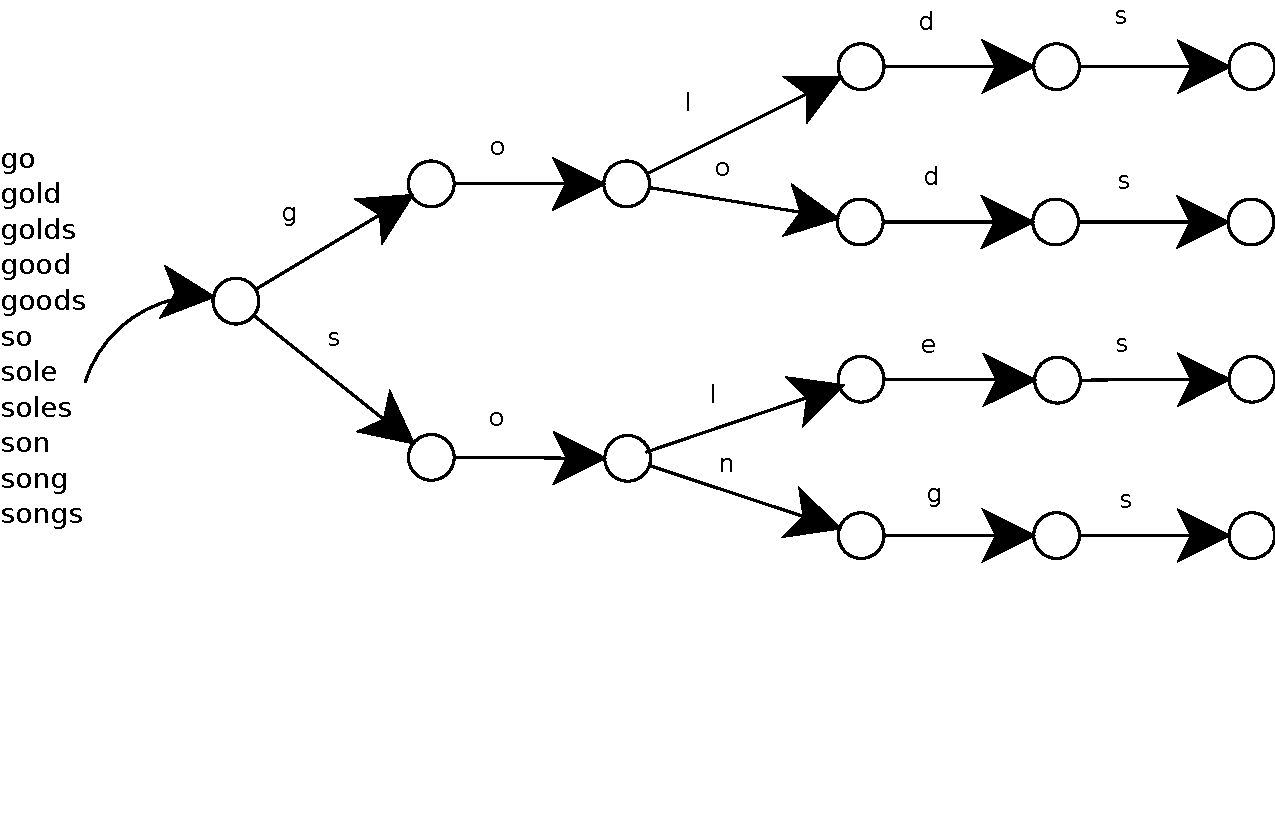
\includegraphics[scale=0.5]{trie}
\caption{Trie. Small dictionary consisting of 11 words represented as a trie.}
\end{figure}
\subsection{Dictionary}
Appel and Jacobsen \cite{fastest} came to the conclusion that a word search will be incredibly fast in a \emph{Directed Acyclic Word Graph}, which in this study will be referred to as a \emph{DAWG}. A DAWG is generally built from a trie, and can be explaind like a minimized trie. Where a trie has a lot of redundancy, becuase of edges and nodes being identical, no such thing occurres in a DAWG. All the identical edges and nodes are removed, and reduced to only one occurancy. As an example in the paper mentioned, the dictionary consisting of more than 100 000 words taking up a memory space of a half mega bytes, could be reduced to occupy only 175 kile bytes.


\subsection{Word generation}
The problem of generating legal moves can be reduces to one dimension. Instead of doing a search in two directions (up and right) it is possible to use an algorithm that generates words only horizontally. The argument is that generating a word vertically is basically the same thing as generating a word horizontally. The only difference is that the board is transposed. Therefore, the algorithm to generate words is limited to only generate horizontally, and for each move we do two searches, where one is over the transposed board.

\subsubsection{Anchor squares}
A key in the algorithm implemented are the \emph{anchor squares}, which are the empy squares next to a non-empty square as can be seen in figure \ref{fig:anchors}. These are important since words can only be built from already existing tiles. In the very forst move there is only one anchor; the center square, since the player making the first move always has to start in the center square.

\begin{figure}
\centering
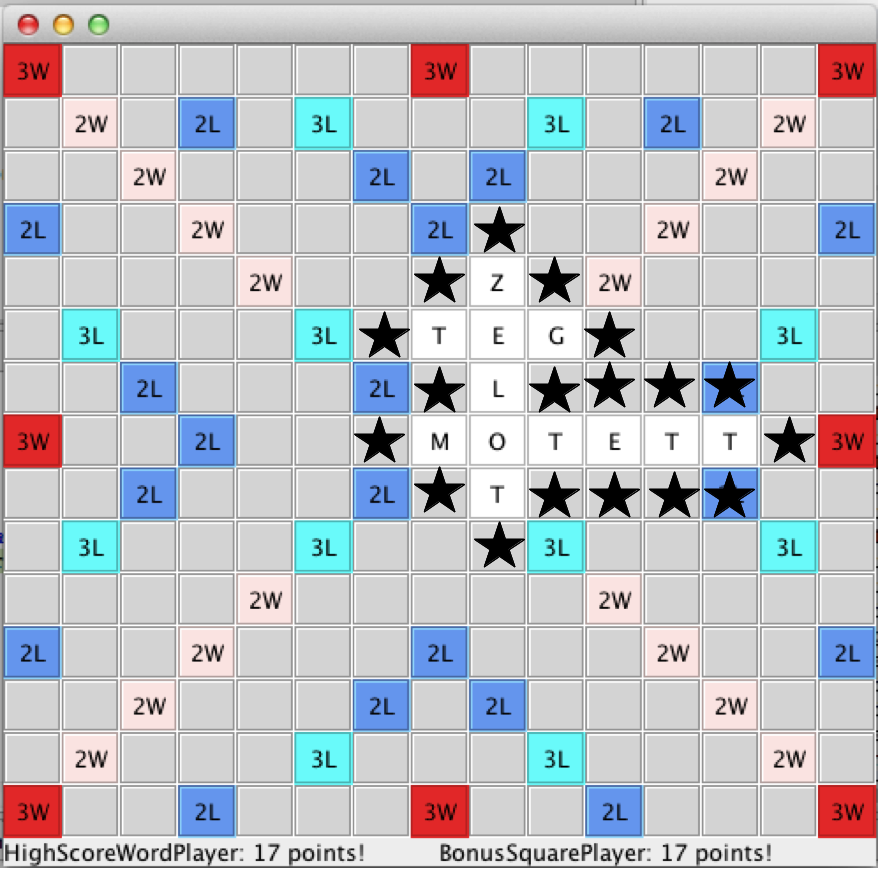
\includegraphics[scale=0.3]{anchors}
\caption{Anchor squares. The adjacent tiles are the anchor tiles from which the word generation begins.}
\label{fig:anchors}
\end{figure}

\subsubsection{Cross-check sets}
When placing a word horizontally, the vertically placed letters also have to create a legal word. It is quite easy to establish that if we place a word horizontally, the vertical word can increas with only one letter at a time. This makes it possible to calculate, for each anchor square, which set of letters that are possible to place at that square. The calculations can be made before each move, and allows the player to place a word by row, without considering the rest of the board. The set of available letter for one square is in Appel and Jacobsen's paper \cite{fastest} referred to as a \emph{cross-check set}

\subsection{Game strategies}
\label{sec:strategies}
If one is a beginner at Scrabble, there are meny small tricks to learn to advance quickly. Some of the tricks can be listed as:

\begin{itemize}
\item Difficult letters. Letters with high score are usually more difficult to place and should be used as soon as possible.
\item Balance on the rack. It is easy to get stuck with only consonants or only vowels on the rack, keeping a good balance can therefore be a good idea to avoid deadlocks in the future.
\item Bonus squares. Hitting the bonus squares can generate a high score. Although it is preferable to avoid opening opportunities for the opponent to do the same.
\item Word extensions. According to Sheppard \cite{perfectgame}, the ability to find extensions (i.e. prefixes and suffixes) to already placed words, is a key to being a successful player since such moves can generate very high scores.
\item Vocabulary. There are many short words in the language, and it is instantly rewarding if a player can learn many short word letters.
\end{itemize}






\chapter{Implementation}
The study is based on an implementation that follows the example of Appel and Jacobsen \cite{fastest}, with some small modifications. Since implementing a DAWG seemed like a time consuming project, a chioce was made to stay with the trie. The advantage with a DAWG is that it saves a lot of memory, but there were no problems with memory space, and therefore an unnecessary thing to focus on.

In the implementation there were some game limitations made to make the study fit into the given time span. The game limitations are described in section \ref{sec:limitations}.

Three different agents were implemented with different strategies to follow and they are all described in section \ref{sec:agents}.

The analysis and the final results are shown in section \ref{sec:analysis}.

\section{Game limitations}
\label{sec:limitations}
To limit the work load to fit into the time span, some limitations were made to the game. This study focuses on games played by only two players, and the implementation is therefore customized to handle only two player games. The players have two options during a turn; either lay a word, or pass the turn and receieve zero points. In other words; the possibility to change tiles if no word can be found is removed. 

The bag is also minimized, and do not contain any blank letters or other special tiles that are not letters. The result is that a Q or a W never can be used. In addition, the game is played in Swedish by the agents.

\section{Agents}
\label{sec:agents}
To see which of the very basic strategies listed in section \ref{sec:strategies} is the most successful one against the others, three agents with different strategies were implemented. The would play against each other in order to generate results for later analyze. This section describes the three different agents implemented, and their strategy in the game. In order to evaluate which strategies are the more rewarding, the agents are implemented with only \emph{one} strategy. An agent who calculates the total score of a move and chooses the highest one will easily win over the tested agents in this study. The agents will be referred to as follows:
\begin{description}
\item{HSW} High score word player.
\item{BS} Bonus square player.
\item{BOR} Balance on rack player.
\end{description}

\subsection{High score words}
One strategy one can use when playing Scrabble is the fact that some letters are more worth than others. These letter are less commonly used in the language and is therefore more difficult to use. Naturally, one would want to use them as soon as there is an opportunity, to not risk getting stuck later in the game. One od the agents tested in this study follows the strategy of placing higher score generating letters first. By all legal moves generated, the agent will chose the one were the word itself has the highest score. 

\subsection{Bonus squares}
Sometimes, it can be more rewarding to place a relatively short word than a longer one. This is because of the bonus squares spread out on the board. The can multiply the value of either one letter, or the entire word placed, and can therefore generate quite high scores. The second agent strives to place words over bonus squares, to hopefully generate a high score. If there are several opportunities to reach a bonus tile, the most rewarding one is chosen by the agent, i.e. the word reaching the bonus square with the highest bonus.

\subsection{Balance on rack}
An important thing to think about when playing Scrabble is to plan for the next move. If a player ends up with only consonants on the rack, the possibility of laying out a word is reduced. The third agent tested tries to always keep a good balance between vowels and consonants on the rack, to avoid deadlocks later in the game. The agent knows the \emph{ideal ratio} and tries to lay out words so that the words left on the rack returns a ratio as close to the ideal ratio as possible. Tests with different ideal ratios are made.

\chapter{Results}
\label{sec:analysis}
Each of the agents has been tested against the others, to let us evaluate the impact of each strategy. Explanations of the agents can be read about in section \ref{sec:agents}. Section \ref{sec:conditions} describes under which conditions the tests were made.

Sections \ref{sec:highBalance}, \ref{sec:balanceBonus} and \ref{sec:bonusHigh} show the results from each run.
 
\section{Test conditions}
\label{sec:conditions}
\subsection{Games}
In one run the agents were set to play 1000 games against each other and to minimize the impact of opening the game in the results, both agents started the game 500 times. Each run were made 10 times, so the total result is based on 10 000 games. It was established that there were no significant changes in the results between running 1000 games, and 10 000 games, and would therefore probably be reduntant to make more tests. 

\subsection{Dictionaries}
Two dictionaries were used in the tests; one consisting of only the normal form of each word and the other consisting of all possible forms of each words, where the latter is a set of 480391 words. The former consists of 83247 words. The rules of Swedish Scrabble do not allow words of all forms, but the english does. Therefore, it seemed interesting to compare how the agents would perform with different conditions. There could be situations where for instance the bonus player has an advantage if conjunctions are allowed, since it strives always after covering the bonus squares. The large dictionary could allow the player to place short extensions to already placed words.

\graphicspath{{../results/Plots/}}
\section{High score words vs Balance on rack}
\label{sec:highBalance}

The results from runs over the large dictionary and the small dictionary do not differ that much, as can be seen in figure \ref{fig:largeDict} and figure \ref{fig:smallDict}.
The BOR player uses a ratio between vowels and consonants on the rack, and strives to keep the ratio after each move. The wanted number of vowels on hand will be referred to as \emph{vowel ratio}. Several tests were made with the BOR player to see if there is any difference when altering the ratio parameter. The ratio is calculated as the number of vowels left on hand divided into the number of consonants left on hand. Table \ref{tab:bor+hsw} shows the results of the runs made with different ideal number of vowels on hand.

The results show that the HSW player is generally more successful playing the game. The BOR player doeas not take the word score in consideration when playing, but only the ratio, and it it obviously not the most rewarding strategy to follow. An interesting observation is that if the BOR agent tries to keep a ratio of vowels close to 1, i.e all tiles being vowels, there is a significant peak in the number of winning games for the agent. On the other hand, trying to keep one vowel on hand after each round seems to not be as smart, since the agent lost almost 100\% of all games.

\begin{table}
\centering
    \begin{tabular}{ | l | l | l | p{5cm} |}
    \hline
   	Vowel ratio & HSW & BOR \\ \hline
	0/8 & 9922 & 73 \\ \hline
    	1/8 & 9999  & 1\\ \hline
    	2/8 & 9484 & 507 \\ \hline
    	3/8 & 9777 & 212\\ \hline
	4/8 & 9735 & 262 \\ \hline
	5/8 & 9627 & 368 \\ \hline
	6/8 & 9146 & 838 \\ \hline
	7/8 & 9863 & 134 \\ \hline
	8/8 & 8762 & 1206 \\ \hline
    \end{tabular}
\caption{Winnings depending on vowel ratio. Amount of winning games of a total of 10 000 games.}
\label{tab:bor+hsw}
\end{table}

\begin{figure}
\centering
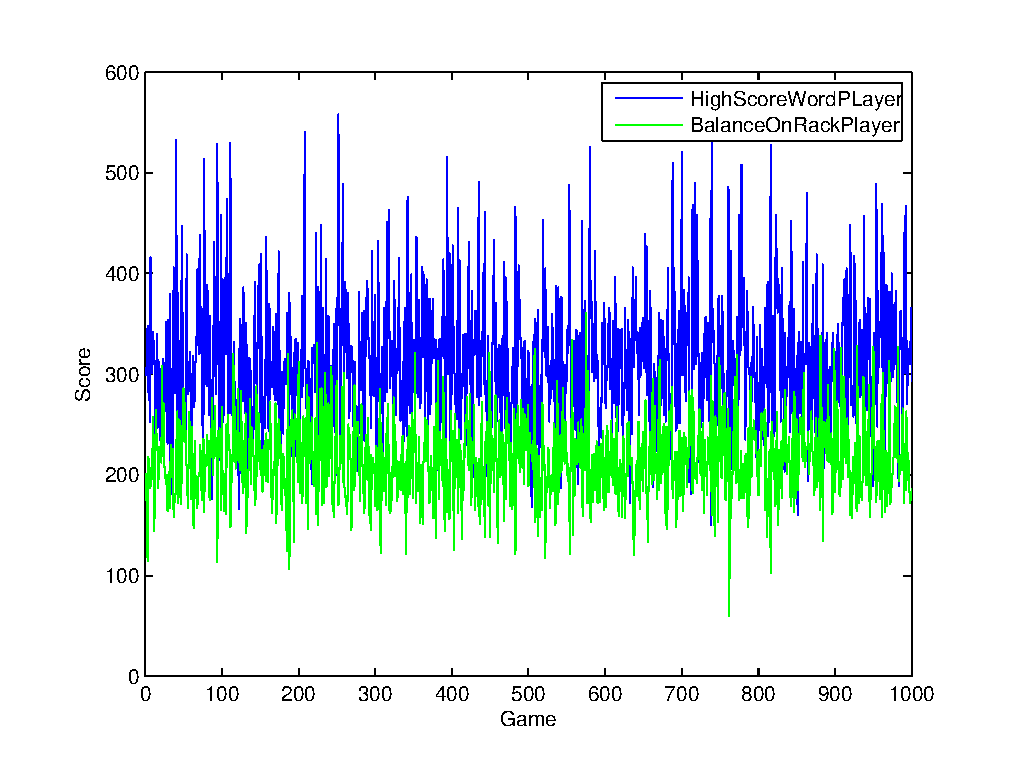
\includegraphics[scale=0.5]{HighBalance8vow}
\caption {Scores with vowel ratio 2/8. Scores of the two players in 1000 games with 480 391 words available.}
\label{fig:smallDict}
\end {figure}

\begin{figure}
\centering
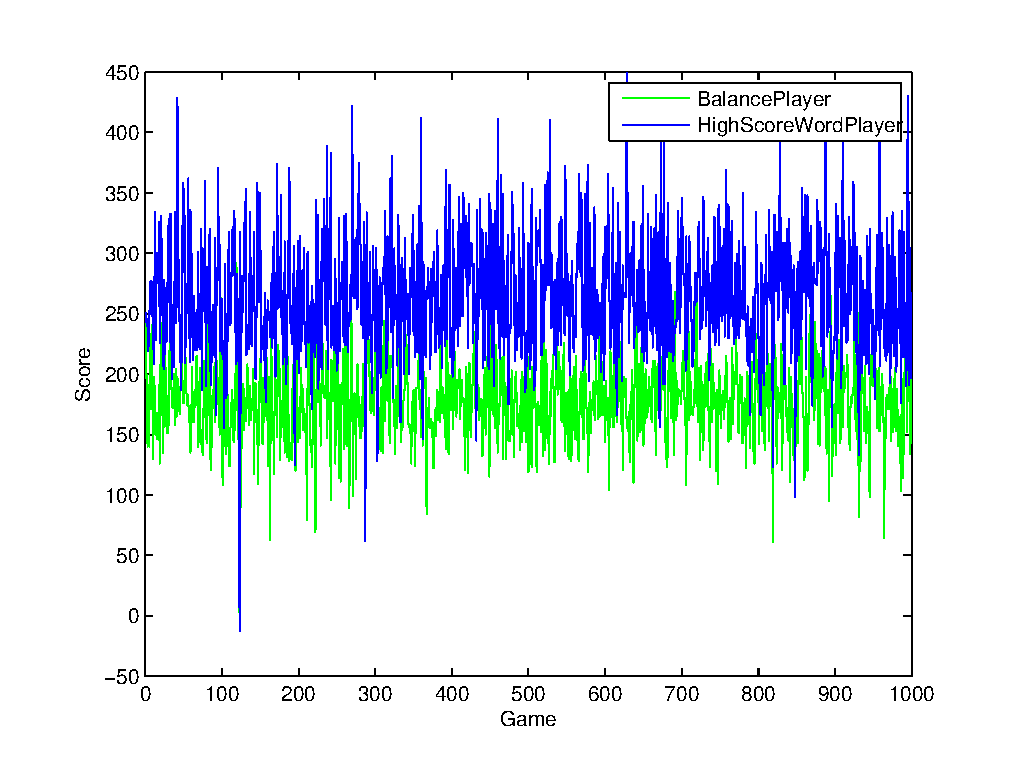
\includegraphics[scale=0.5]{High_Balance2pen2vow_1000games_smallDict}
\caption {Scores with vowel ratio 2/8. Scores of the two players in 1000 games with 83 247 words available.}
\label{fig:largeDict}
\end{figure}

\section{Balance on rack vs Bonus squares}
\label{sec:balanceBonus}
The BOR player continues to perform doubtly against the BS player. Also here the BS player consideres what bonus it will be given in a certain move, and chooses the highest one. Naturally the BOR player that only cares about its ratio on the rack will perform worse. The results from runs with different vowel ratio in the BOR player can be seen in table \ref{tab:bor+bs}.

Note that the BOR player is stable with its game results. In figure \ref{fig:bonusBalanceLargeDict} one can see that the BS player in some games made an extremely poor performance, receiving zero points or less, while the BOR player keeps the graph quite thin, i.e. the results differ less from game to game.

\begin{table}
\centering
    \begin{tabular}{ | l | l | l | p{5cm} |}
    \hline
   	Vowel ratio & HSW & BOR \\ \hline
	0/8 & 0 & 0 \\ \hline
    	1/8 & 0 & 0 \\ \hline
    	2/8 & 0 & 0 \\ \hline
    	3/8 & 0 & 0 \\ \hline
	4/8 & 0 & 0 \\ \hline
	5/8 & 9731 & 261 \\ \hline
	6/8 & 9370 & 620 \\ \hline
	7/8 & 9859 & 141 \\ \hline
	8/8 & 9074 & 915 \\ \hline
    \end{tabular}
\caption{Winnings depending on vowel ratio. Amount of winning games of a total of 10 000 games.}
\label{tab:bor+bs}
\end{table}

\begin{figure}
\centering
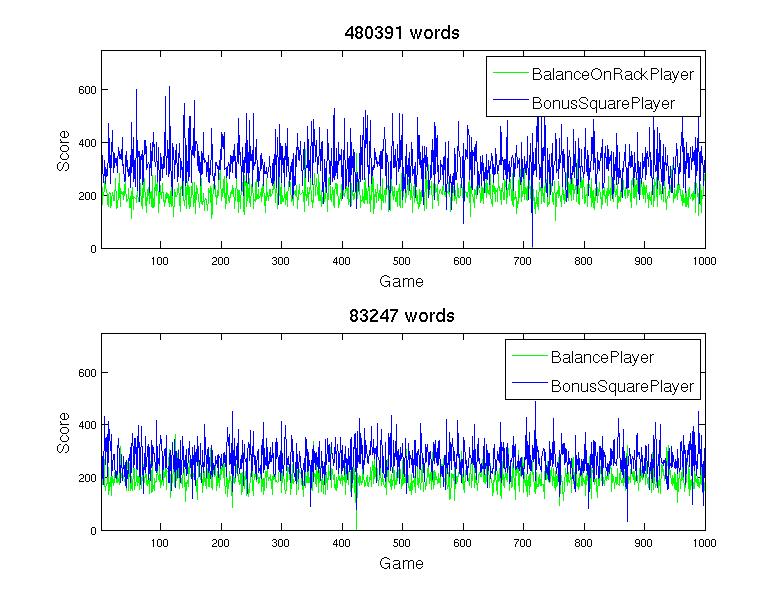
\includegraphics[scale=0.5]{BonusBalance8vow}
\caption {Scores with vowel ratio 2/8. Scores of the two players in 1000 games with 83 247 words available.}
\label{fig:bonusBalanceLargeDict}
\end{figure}


\section{Bonus squares vs High score words}
\label{sec:bonusHigh}
The results from games go here.




\chapter{Conclusions}
\subsubsection{BOR player}
The BOR player is significantly better with a vowel ratio of 8/8. It can probably be explained from the fact that when choosing a move, and the vowel ratio is 8/8 (1) it is easier for the agent to place longer words. Imagine the agent placing a word using all tiles but one, and the remaining tile on hand is a vowel. This would be a preferable move if the ratio is 1, but not if the ratio is less. If the ratio would be 4/8 for example, the agent would choose a move that leaves two tiles, where one is a vowel, over the move with a longer word. 






\begin{thebibliography}{100}  
  \bibitem{perfectgame} Sheppard, B., 2002, Towards Perfect Play of Scrabble, Maastricht.
  \bibitem{fastest} Appel A. W., Jacobson, G. J., 1985, The World’s Fastest Scrabble Program, Commun. ACM, 31(5), 572-585, May 1988.
\bibitem{faster} Gordon, S. A., 1993, A Faster Scrabble Move Generation Algorithm, Software - Practice and experience, Vol. 24(2), 219-232, February 1994.
\bibitem{quakle} Katz-Brown, J., O’Laughlin, J., Fultz, J., Liberty, M., Buddhdev, A., 2006, Quakle - open source crossword game software, http://people.csail.mit.edu/jasonkb/quackle/, 2 January 2012,  12 February 2012.
\bibitem{scrabblewiki} Wikipedia, Scrabble, http://en.wikipedia.org/wiki/Scrabble, 12 February 2012.
\bibitem{frank} Andersson, G., Ivansson, L., Frank - crossword software game, http://ivansson.org/Frank/, 22 August 2009, 12 February 2012.
\bibitem{wordfeud} Hbwares, Wordfeud, http://www.wordfeud.com, September 2010, 12 February 2012.
\bibitem{ai} Russell S., Norvig P. Artificial Intelligence: A Modern Approach 3rd ed. Prentice Hall. 2009
\bibitem{inforetrieve} Manning C. D., Raghavan P., Schütze H., Introduction to Information Retrieval, Cambridge University Press, 2008, p. 49-65.
\bibitem{forbund} Svenska Scrabbleförbundet, www.scrabbleforbundet.se.
\end{thebibliography}
\end{document}